\documentclass[hyperref={unicode}]{beamer}
%
% Choose how your presentation looks.
%
% For more themes, color themes and font themes, see:
% http://deic.uab.es/~iblanes/beamer_gallery/index_by_theme.html
%
\mode<presentation> {
	\usetheme{Berkeley}      % or try Darmstadt, Madrid, Warsaw, ...
	\usecolortheme{seahorse} % or try albatross, beaver, crane, ...
	\usefonttheme{default}  % or try serif, structurebold, ...
	\setbeamertemplate{navigation symbols}{}
%	\setbeamertemplate{caption}[numbered]
	\setbeamertemplate{caption}{\raggedright\insertcaption\par}		
	% Numbered bibiolgraphy items
%	\setbeamertemplate{bibliography item}{\insertbiblabel}
} 

\usepackage[utf8]{inputenc}
\usepackage[english]{babel}
\usepackage[T1]{fontenc}
\usepackage{csquotes,lmodern,silence}
%\usepackage[style=numeric,backend=biber]{biblatex}

%\WarningFilter{biblatex}{Patching footnotes failed}

% Remove small caps warning
%\renewcommand\mkbibacro[1]{{\footnotesize\MakeUppercase{#1}}}

%\addbibresource{bibliography.bib}
\graphicspath{{figures/}}

\title[Linux Boards]{Linux boards and their use}
\author{Peter Babič}
\institute{Technical University of Košice, Slovakia \\ Computer Modelling, Masters}
\date{26.11.2015}

\begin{document}

\titlepage

%\begin{frame}{Talk Outline}
%  \tableofcontents
%\end{frame}



\section{Introduction}

\begin{frame}{Introduction}
	What is a Linux board? Where did it come from?
	\begin{figure}
	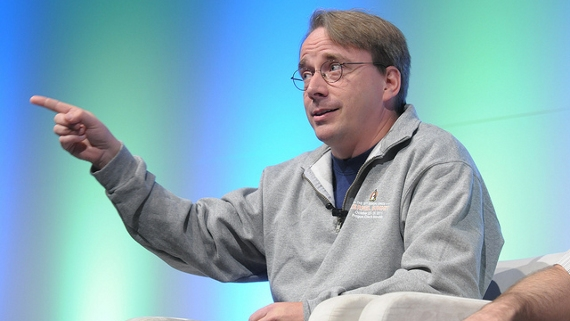
\includegraphics[width=.7\textwidth]{linus-torvalds-linuxcon.jpg}
	\caption{I don't have time for this!}
	\end{figure}
\end{frame}


\section{Boards}





\subsection{Single Board Computers}

\begin{frame}{Single Board Computer}
\begin{figure}
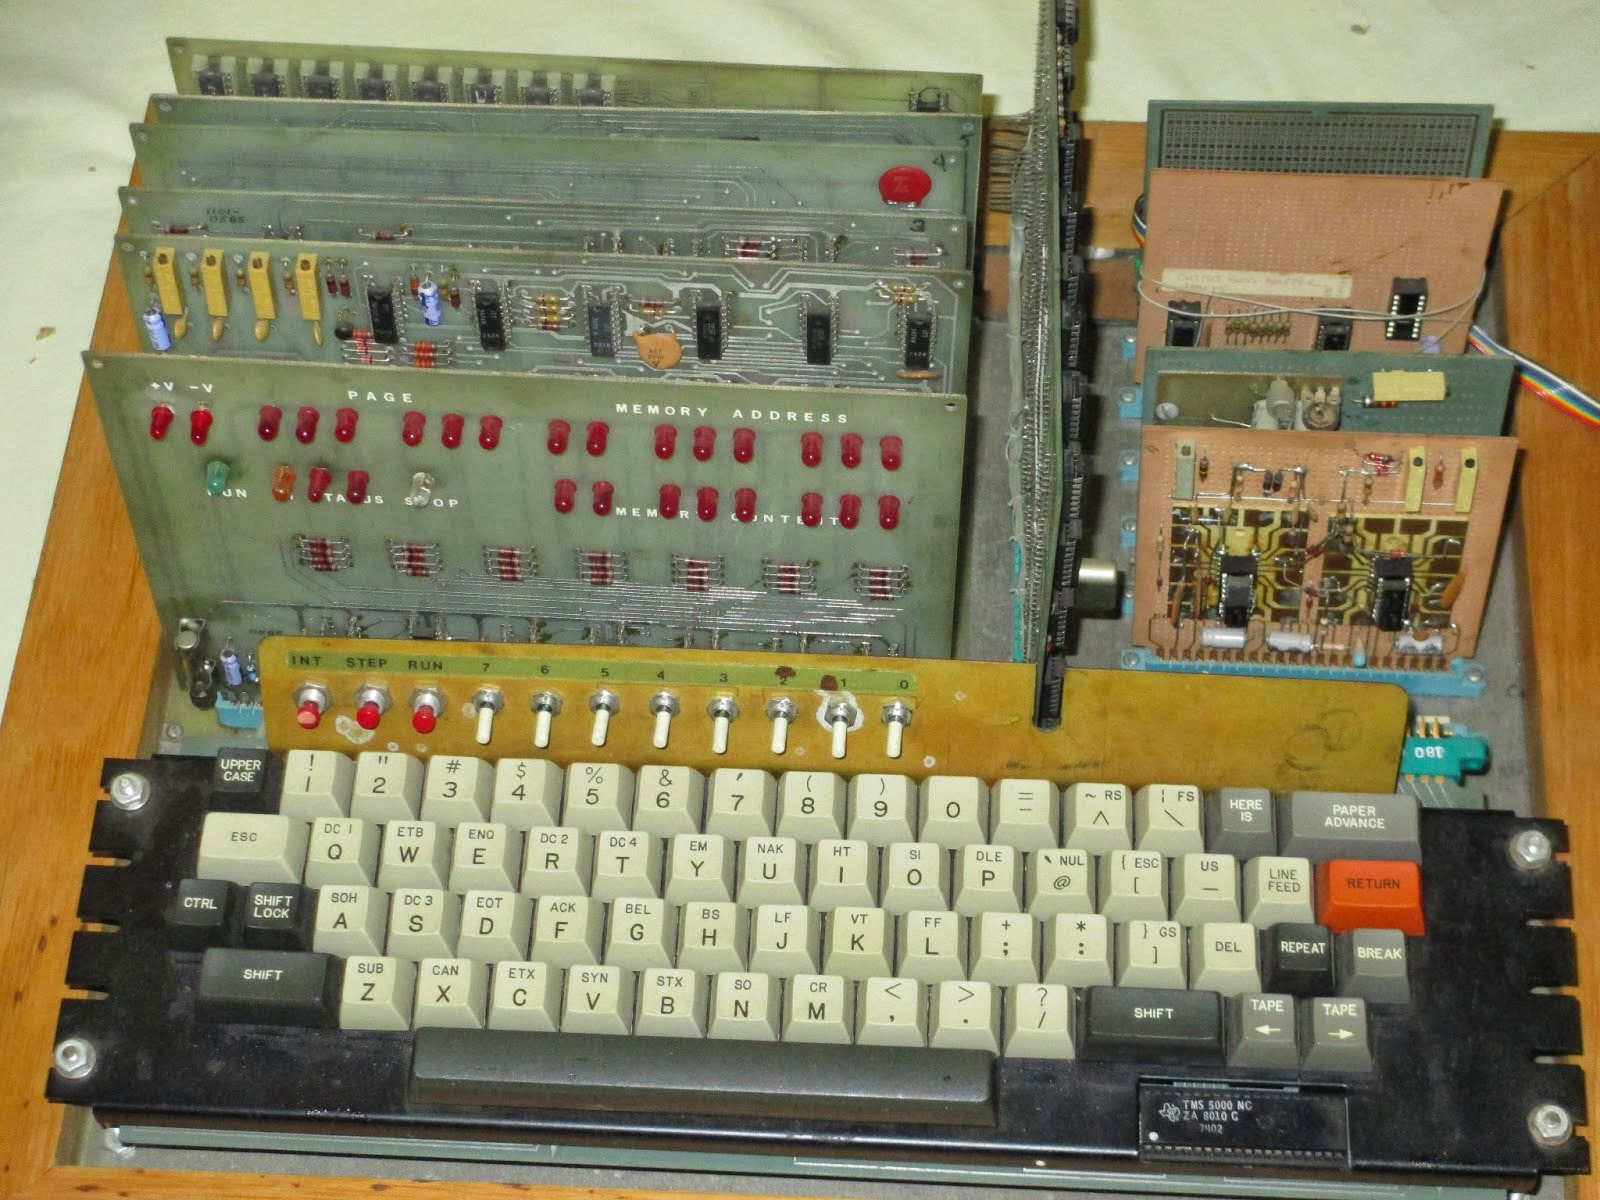
\includegraphics[width=.7\textwidth]{scelbi.jpg}
\caption{A "single board" computer}
\end{figure}
\end{frame}

\subsubsection{Pioneers}

\begin{frame}{SBC Pioneers}
\centering
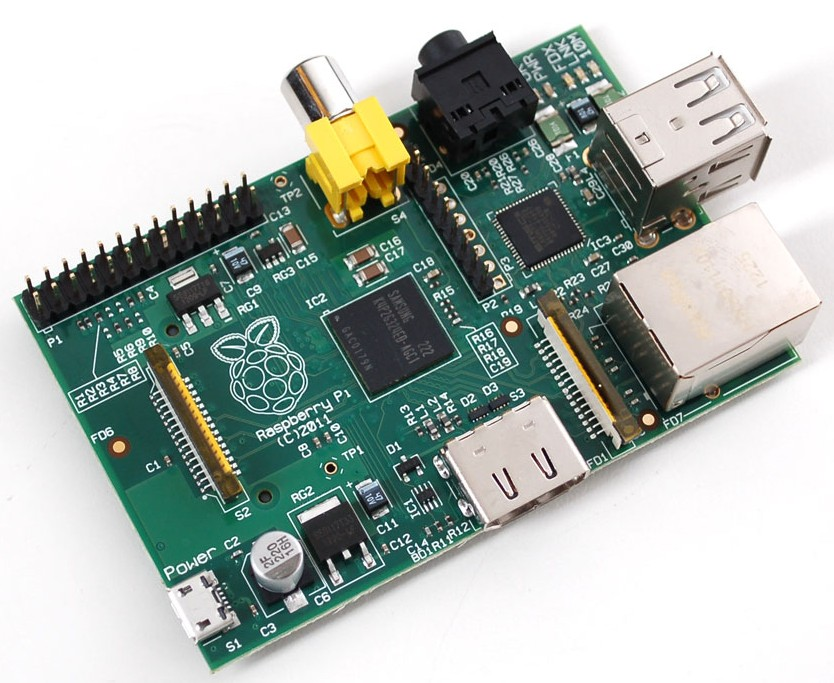
\includegraphics[width=.40\linewidth]{raspi.jpg}
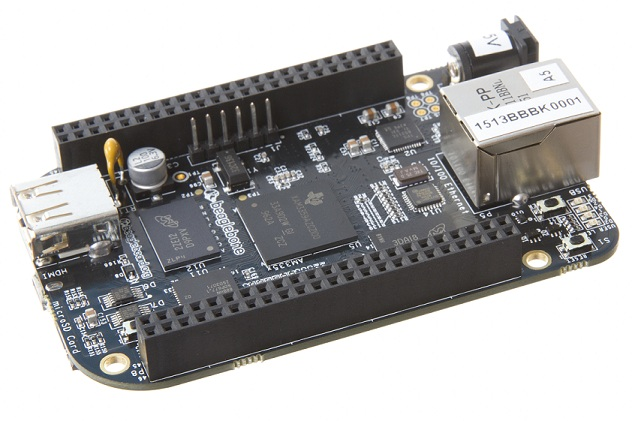
\includegraphics[width=.40\linewidth]{beagle.jpg}
\newline
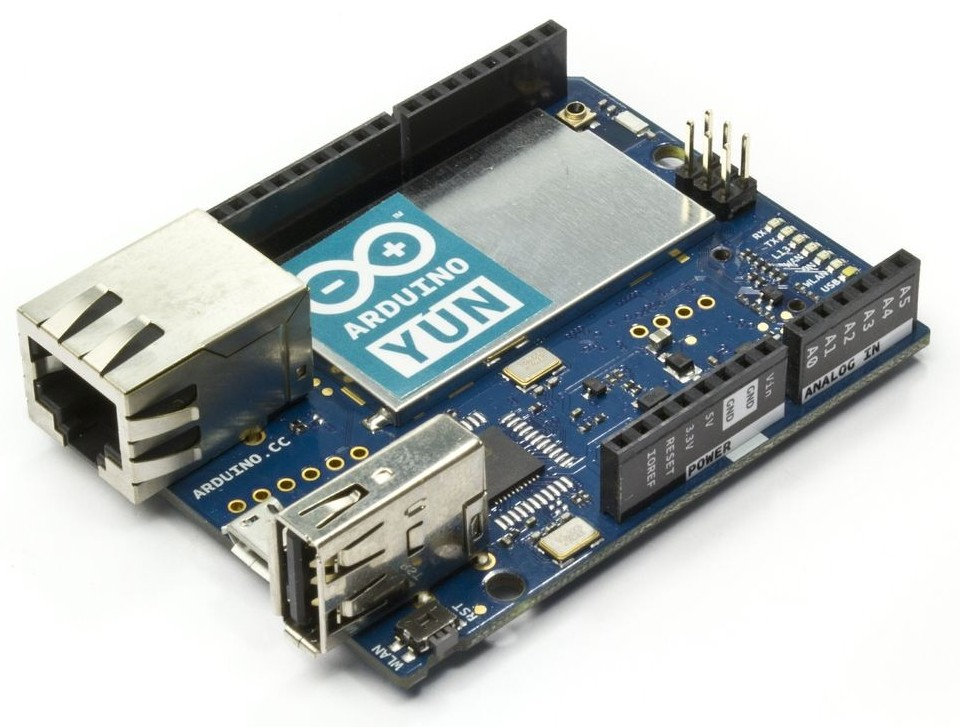
\includegraphics[width=.40\textwidth]{arduino-yun.jpg}
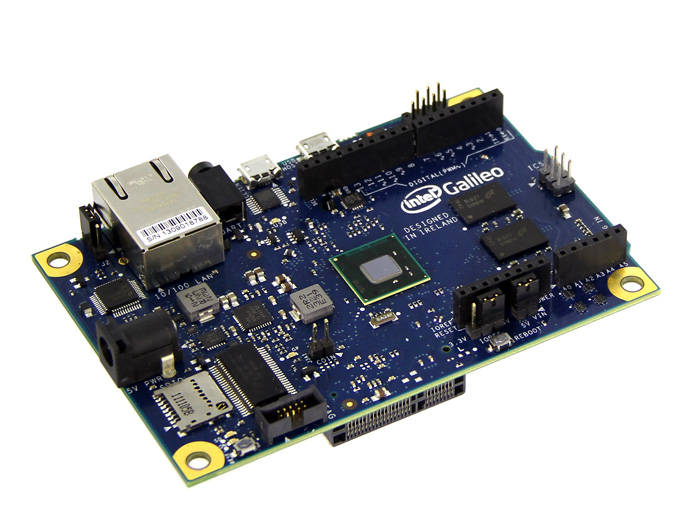
\includegraphics[width=.40\textwidth]{galileo.jpg}
\end{frame}


\subsubsection{Projects}

\begin{frame}{Why are SBC useful?}
\begin{figure}
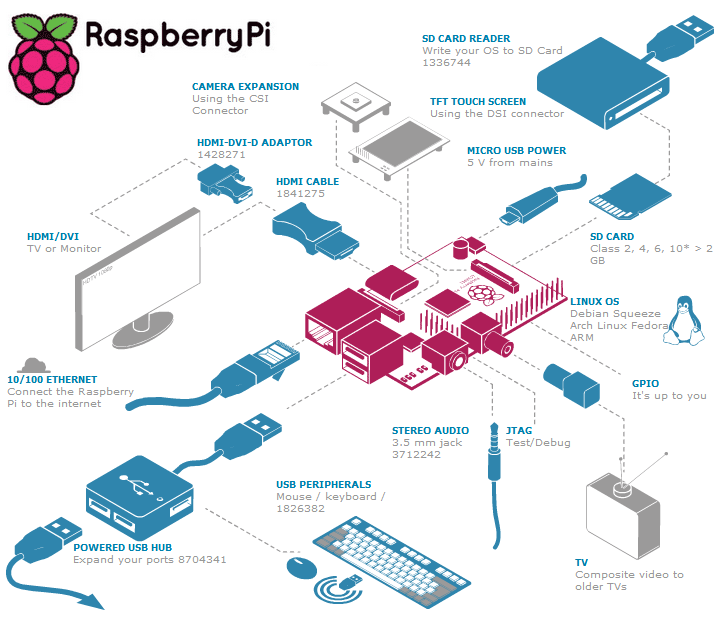
\includegraphics[width=.7\textwidth]{raspi-peripherals.png}
\caption{Raspberry Pi with a range of available peripherals}
\end{figure}
\end{frame}


\begin{frame}{Done by others}
	\begin{itemize}
	\item CNC and 	3D printer controllers
	\item Clusters, parallel computers	
	\item Handheld game devices
	\item Computer console emulators (MAME)
	\item Vending machine controllers
	\item Various robots
	\item Bitcoin miners
	\item Educational tools
	\end{itemize}
\end{frame}



\subsection{Embedded}

\begin{frame}{Embedded Computing}
	\begin{figure}
	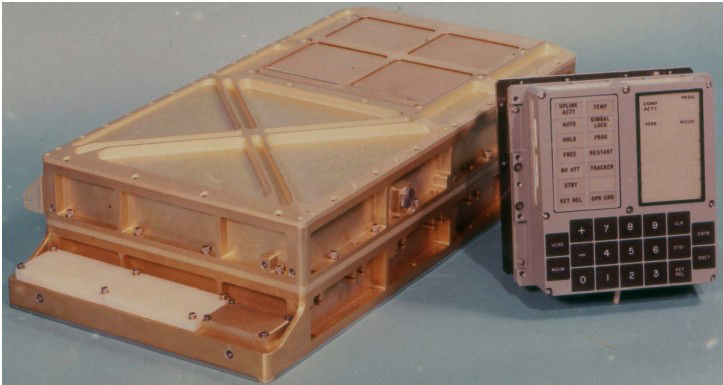
\includegraphics[width=.8\textwidth]{apollo-guidance.jpg}
	\caption{Apollo Guidance Computer and Numeric Display with a Keyboard}
	\end{figure}
\end{frame}


\subsubsection{Common Boards}

\begin{frame}{Cheap and Common Embedded Boards}
	\centering
	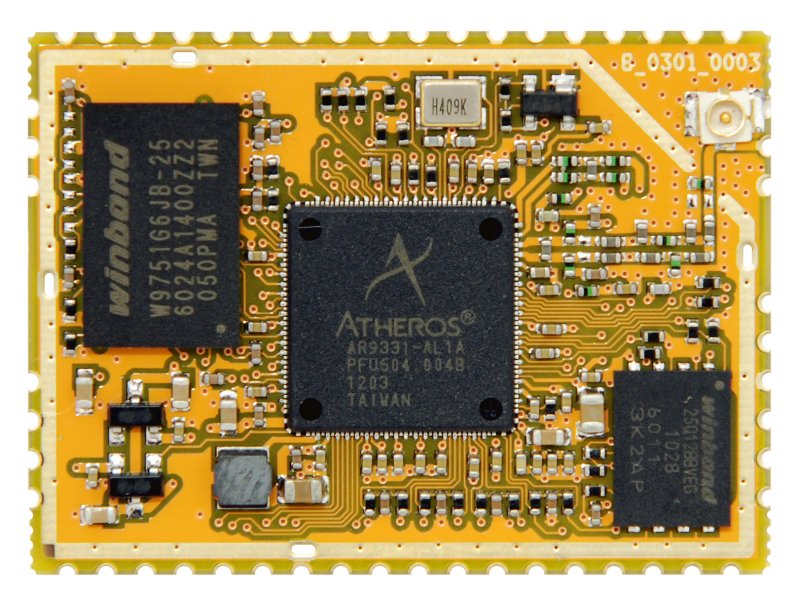
\includegraphics[width=.40\linewidth]{carambola2.png}
	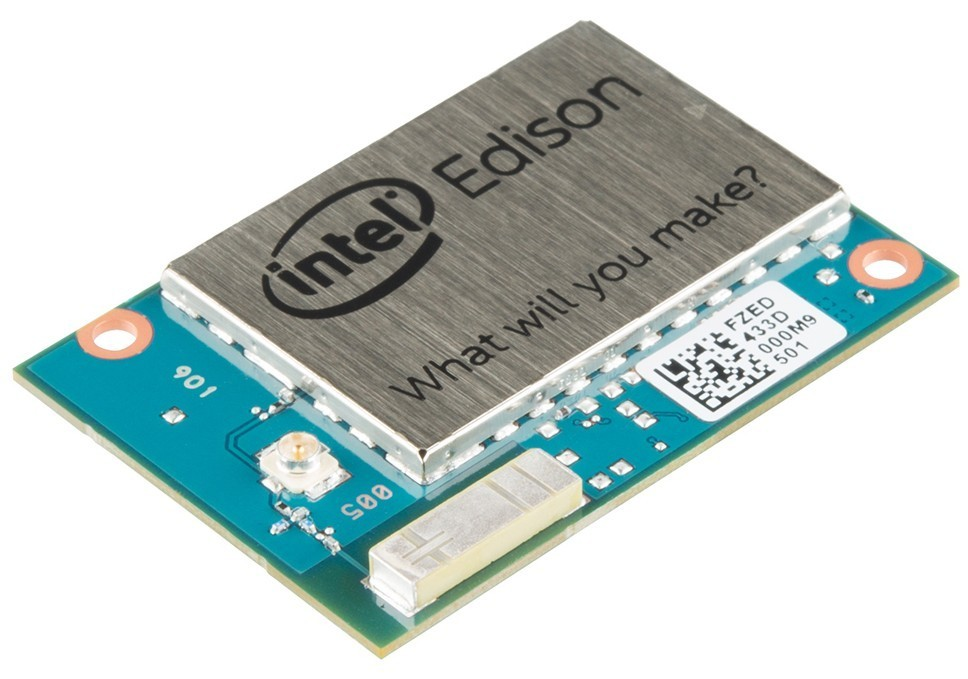
\includegraphics[width=.40\textwidth]{intel-edison.jpg}
	\vskip 1cm
	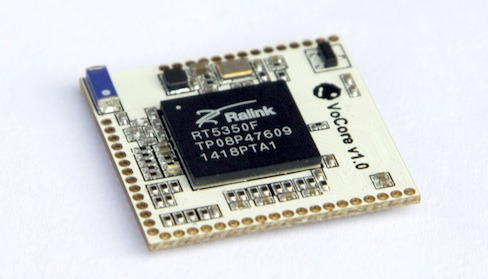
\includegraphics[width=.40\linewidth]{vocore.jpg}
	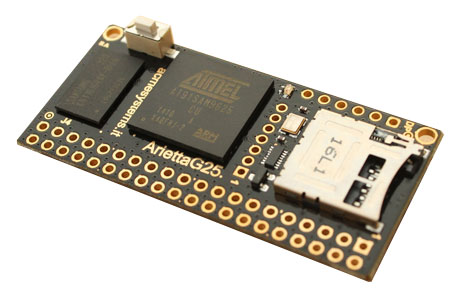
\includegraphics[width=.40\textwidth]{arietta-g25.jpg}
\end{frame}

\subsubsection{GL-Inet}

\begin{frame}{GL-Inet Smart Router}
	\begin{figure}
	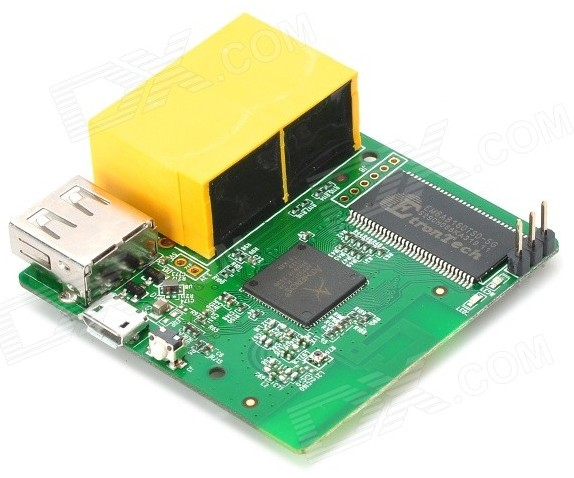
\includegraphics[width=.7\textwidth]{glinet.jpg}
	\caption{The personal pavorite number 1}
	\end{figure}
\end{frame}


\begin{frame}{TP-Link WR703n}
	\begin{figure}
	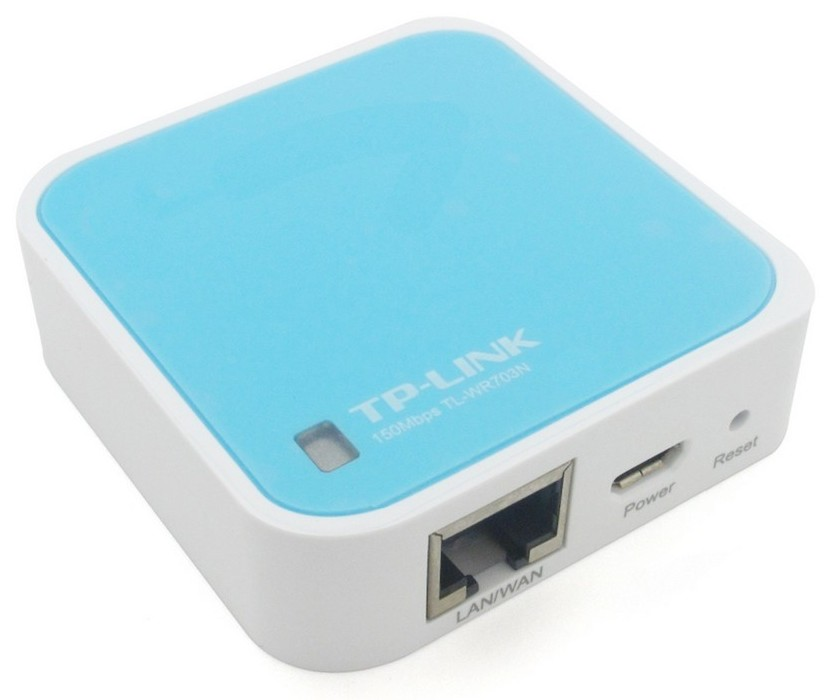
\includegraphics[width=.7\textwidth]{wr703n.jpg}
	\caption{The predecessor of a GL.Inet}
	\end{figure}
\end{frame}


\section{Opereating system}

\begin{frame}{Why Linux?}
	\begin{figure}
	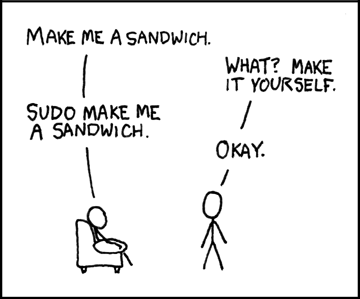
\includegraphics[width=.7\textwidth]{sandwich.png}
	\caption{Randall Munroe knew it before}
	\end{figure}
\end{frame}

\subsection{Linux}

\begin{frame}{The Linux Ecosystem}
	\begin{figure}
	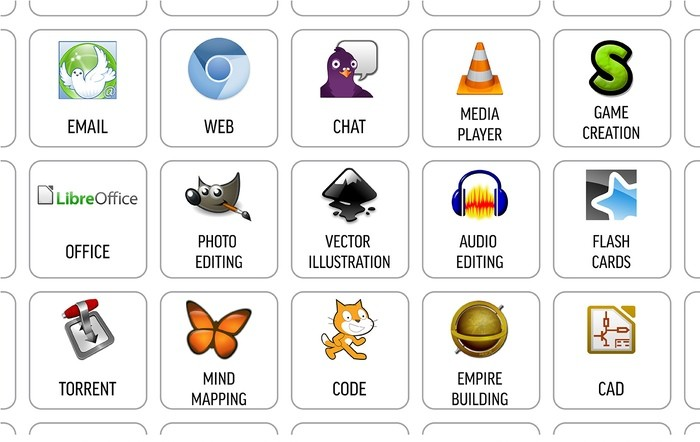
\includegraphics[width=.75\textwidth]{linux-apps.jpg}
	\caption{Marketing says: IT'S ALL FREE!}
	\end{figure}
\end{frame}

\subsection{OpenWRT}

\begin{frame}{OpenWRT}
	\centering
	
	\begin{block}{Question}
	What can you do with a full blown Linux, given only 16MB, 8MB or even 4MB RAM or Flash is available?
	\end{block}
	
	\vskip .4cm
	\begin{figure}
	
\includegraphics[width=.4\textwidth]{busybox.png}
	\caption{BusyBox (+ uClibc)}
	\end{figure}	

\end{frame}



\section{The Future}


\begin{frame}{Where is it all going?}
	\begin{figure}
	
\includegraphics[width=.4\textwidth]{hacked.png}
%	\caption{Security or Privacy, anyone?}
	\end{figure}
\end{frame}


\subsection{IoT}

\begin{frame}{Internet of Things}
	\begin{block}{Definition}
	A network of physical objects or “things” embedded with electronics, software, sensors and connectivity to enable it to achieve greater value and service by \textbf{exchanging data with the manufacturer}, operator and/or other connected devices.
	\end{block}
\end{frame}


\section{Epilogue}

\begin{frame}{Epilogue}
	\centering
	{\large Thank you}
	
	\vskip 2cm
	Peter Babič	

\end{frame}


\end{document}


